\documentclass{article}%
\usepackage[T1]{fontenc}%
\usepackage[utf8]{inputenc}%
\usepackage{lmodern}%
\usepackage{textcomp}%
\usepackage{lastpage}%
\usepackage{authblk}%
\usepackage{graphicx}%
%
\title{Ellipticine{-}induced apoptosis depends on Akt translocation and signaling in lung epithelial cancer cells}%
\author{William Ramirez}%
\affil{Advanced Laboratory for Plant Genetic Engineering, Advanced Technology Development Centre, Indian Institute of Technology Kharagpur, Kharagpur, India}%
\date{01{-}01{-}2014}%
%
\begin{document}%
\normalsize%
\maketitle%
\section{Abstract}%
\label{sec:Abstract}%
Tripoli and Center on Global Health\newline%
Until about two months ago, the lead physician in the Fatema Clinical trial of rheumatoid arthritis (MANA) was the only doctor on the dietician's list. But when the study was launched back in July, the only doc on the exam table was Dr. Sharif Muahed, but Dr. Muahed wasn't satisfied by what he found. He found rheumatoid arthritis and advanced clinical symptoms with elevated liver cells. Now the head physician at MD Anderson Cancer Center, Muahed is eager to add a third doctor to the dieticians' list.\newline%
"We're moving toward increasing the level of research and studies to determine that they have significant potential benefit," says Muahed. "Then we're taking steps toward educating clinicians about the genetic component of the disease."\newline%
Initially, Muahed saw nothing wrong with the men living with advanced clinical signs of advanced disease, but as he prepared for patient conference, he noticed a pattern emerging. Looking through his biopsy books, he found an order manifest for three out of the four liver proteins from liver cells expressing the RA gene sequence. In order to activate the RA gene in patients, there is no active panel for liver enzymes. He researched genetics and came up with a virus theory that does not involve virus, but genetic mutations in the RNA itself of the virus.\newline%
"This whole problem can be solved if we can understand this other mutation and isolate it and diagnose it," he said.\newline%
The second surgery to treat advanced rheumatoid arthritis was a success. Several weeks later, Muahed will deliver the diagnosis and find the genetic mutation. There is a possibility of a colon stone or a blocked intestine that may cause the disease. Now, Muahed's main interest is in making treatments more effective. He's not sure how quickly the cure for advanced disease will be created, but he has the same goal as Sir Francis Collins when he was appointed as the director of the National Institutes of Health (NIH): "It's going to take patients and doctors more persistence in trying to prevent this from happening."

%
\subsection{Image Analysis}%
\label{subsec:ImageAnalysis}%


\begin{figure}[h!]%
\centering%
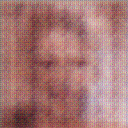
\includegraphics[width=150px]{500_fake_images/samples_5_31.png}%
\caption{A Black And White Photo Of A Black And White Cat}%
\end{figure}

%
\end{document}